%% This is a sample file demonstrating the use of IJCAS.cls,
%% which is for the IJCAS (International Journal of Control, Automation, and Systems).
%%
%% 2004/03/08 by Karnes Kim
%% 2011/07/26 by CDSL, SNU
%%
%% Support sites: http://www.ijcas.com
%%
%% This code is offered as-is - no warranty - user assumes all risk.
%% Free to use, distribute and modify.
%%

%% The IJCAS class supports two column page basically. 
%%So, you need not use two column option or command.
\documentclass{IJCAS}

%% include the useful LaTeX packages:
\usepackage{url}
\usepackage{array,tabularx}
\usepackage{multicol} 
\usepackage{stfloats}

%%%% Editorial Information
%% Authors do not have to modify this section.
\journalvolumn{VV}
\journalnumber{X}
\journalyear{YYYY}
\setarticlestartpagenumber{1}
%%%% End of Editorial Information

%The environment for theorem, lemma, remark, corollary, proposition, and definition are already defined.


%The following command is needed for line break of long equations.
\allowdisplaybreaks


\begin{document}
% the \title command
\title{Vision-Based 2D Scan Generation for Obstacle Avoidance Using Floor Segmentation}

% the \author command
% the \orcid{orcid number}
\author{Hyunseo Lee\orcid{0009-0004-8217-7201}, Gunmin Yoo\orcid{0009-0001-6453-8075}, Hyunwoo Gu\orcid{0009-0008-2779-648X}, and Sung Soo Hwang*\orcid{0000-0002-0863-7503}}

% the abstract environment
\begin{abstract}
We present a vision-based method for generating 2D scan-like data for indoor autonomous mobile robots (AMRs) using a monocular camera. The method uses a lightweight floor-segmentation model to identify traversable regions in RGB images and projects non-floor pixels into approximate range and bearing values through precomputed lookup tables (LUTs) derived from the camera's intrinsic parameters. To reduce the influence of irrelevant image regions, traversability is evaluated within a predefined region of interest (ROI) in front of the robot. The generated scan is formatted as a ROS 2 laser-scan-compatible message and integrated with the Nav2 stack. Experiments in a structured indoor corridor show that the proposed scan can provide usable obstacle cues for a single static frontal obstacle: the robot completed 39 out of 50 trials over a 10-meter path. These results suggest that monocular virtual scanning can serve as a lightweight sensing option for constrained indoor scenarios, while further work is needed to improve robustness under reflective floors, illumination changes, and more diverse obstacle conditions.
\end{abstract}

\begin{keywords}
Floor segmentation, indoor autonomous mobile robot, lightweight sensing, monocular camera, obstacle avoidance, ROS 2 and Nav2 integration, vision-based 2D scan.
\end{keywords}

\maketitle

\makeAuthorInformation{
Manuscript received January 10, 2026; revised March 10, 2026; accepted May 10, 2026. Recommended by Associate Editor Soon-Shin Lee under the direction of Editor Milton John.\\

Hyunseo Lee is with the School of Artificial Intelligence, Computer and Electrical Engineering, Handong Global University, 558 Handong-ro, Pohang 37554, Republic of Korea (e-mail: hslee@handong.ac.kr). Gunmin Yoo and Hyunwoo Gu are with the Department of Computer Science and Electronic Engineering, Handong Global University, 558 Handong-ro, Pohang 37554, Republic of Korea (e-mails: \{gunminy, 21800030\}@handong.ac.kr). Sung Soo Hwang is a Professor with the School of Artificial Intelligence, Computer and Electrical Engineering, Handong Global University, Pohang 37554, Republic of Korea (e-mail: sshwang@handong.edu).

* Corresponding author.
}

\runningtitle{2026}{Hyunseo Lee, Gunmin Yoo, Hyunwoo Gu, and Sung Soo Hwang}{Vision-Based 2D Scan Generation for Obstacle Avoidance Using Floor Segmentation}{xxx}{xxxx}{x}



\raggedbottom
\section{INTRODUCTION}\label{sec1}

Autonomous mobile robots are becoming common in structured indoor settings such as warehouses, hospitals, and offices. Their growth is supported by advances in perception and planning, but practical deployment still faces sensing-related limitations.

Many systems depend on depth sensors, which provide precise spatial data but increase cost, payload, and integration effort~\cite{gvrnextgenerationtechnologiesresearchteam_2026_autonomous,liu_2024_a}. Indoor scenes also contain narrow corridors, glass, polished floors, changing illumination, and sudden obstacles; these factors require responsive sensing but can degrade optical or range measurements~\cite{yang_2019_semantic,deepthadamodaran_2023_experimental,yang_2011_on,tibebu_2021_lidarbased,mei_2021_depthaware,sajjan_2020_clear}.

Combining multiple sensors can improve robustness, but it also increases calibration effort, computation, and tuning complexity~\cite{liu_2024_a,singh_2019_multidata}. In contrast, monocular vision is lighter and easier to integrate, especially for small or low-cost platforms.

Recent segmentation and geometry-inference methods can detect floor regions or infer spatial layout from a single image~\cite{shariqfarooqbhat_2021_adabins,ranftl_2021_vision,ultralytics_2024_ultralytics}. However, vision outputs are not usually produced in the range-message form expected by navigation modules. Real-time middleware integration therefore requires attention to message format, timing, and costmap compatibility~\cite{macenski_2022_robot,macenski_2020_the,openrobotics_sensor_msgslaserscan,opennavigationllc_2023_costmap}.

This paper proposes a lightweight virtual scan generator that segments the floor in monocular images and projects non-floor pixels into a ROS 2 laser-scan-compatible format. Experiments in structured indoor environments show that the generated scan can provide coarse obstacle cues under constrained conditions, including a static frontal obstacle scenario without a dedicated range sensor.

This work provides a practical integration framework that converts floor-segmentation outputs into ROS 2 laser-scan-compatible observations. Specifically, the proposed system maps segmentation outputs into laser-scan-like obstacle observations through camera-calibrated LUTs, validates forward traversability within a task-specific ROI, and integrates the resulting scan with Nav2 costmaps for real-time obstacle avoidance. The study also provides an empirical evaluation of the approach through range-estimation tests and repeated 10-meter navigation trials, clarifying both its usefulness and its current limitations in structured indoor environments.

The remainder of this paper is organized as follows. Section~\ref{sec2} reviews related work and technical challenges. Section~\ref{sec3} presents the proposed method. Section~\ref{sec4} reports experimental results, and Section~\ref{sec5} concludes the paper.

\section{RELATED WORK AND TECHNICAL CHALLENGES}\label{sec2}

LiDAR and other active range sensors are widely used for mapping, localization, and obstacle detection because they provide direct geometric measurements for occupancy-grid and navigation pipelines~\cite{li_2020_lidar,yusuf_2022_iotbased,liu_2024_a}. However, active sensors increase cost, payload, power consumption, and integration effort, which can be restrictive for small indoor AMRs~\cite{gvrnextgenerationtechnologiesresearchteam_2026_autonomous,liu_2024_a}. Their measurements are also not failure-free: glass, mirrors, glossy floors, and other specular or transparent surfaces can create missing returns, false structures, or distorted occupancy maps~\cite{deepthadamodaran_2023_experimental,yang_2011_on,wang_2017_detecting,tibebu_2021_lidarbased}. These limitations motivate lighter sensing configurations for structured indoor environments, provided that their uncertainty is made explicit and their navigation role is evaluated conservatively.

Vision-based alternatives address part of this need because cameras are compact, inexpensive, and already common on mobile platforms. Monocular approaches have been used to estimate depth, infer dense scene geometry, or classify traversable regions from a single RGB stream~\cite{shariqfarooqbhat_2021_adabins,ranftl_2021_vision,wang_2021_a,dang_2023_obstacle}. Segmentation models such as the Ultralytics YOLO11 family also make it practical to extract task-specific regions, including floor areas, at low computational cost~\cite{ultralytics_2024_ultralytics}. Nevertheless, monocular perception remains coupled to appearance: illumination, floor reflectance, shadows, mirrors, transparent objects, scene layout, and training-data coverage can all affect free-space stability~\cite{mei_2021_depthaware,sajjan_2020_clear,deepthadamodaran_2023_experimental,singh_2019_multidata}. A monocular system should therefore define a constrained operating condition and translate its visual output into a form that downstream navigation software can use safely.

Most vision-based navigation studies emphasize the perception model itself, such as depth estimation accuracy, obstacle classification, or free-space segmentation. These outputs are useful, but they are not automatically compatible with mature mobile-robot navigation stacks. Dense monocular depth maps often require additional filtering and geometric calibration before they can be used as planar obstacle observations, while semantic masks provide class information without direct range values. Conversely, scan-conversion tools in ROS usually assume that depth images or point clouds are already available~\cite{openrobotics_2020_depthimage_to_laserscan,openrobotics_2015_pointcloud_to_laserscan}. This leaves a practical gap for low-cost AMRs that only carry a monocular RGB camera: visual traversability cues must be converted into a time-stable, range-like representation before they can affect local planning in a predictable way.

This perception-navigation interface is a central technical issue. Modern mobile robots commonly rely on ROS and ROS 2 middleware for perception, planning, and control~\cite{quigley_2009_ros,macenski_2022_robot}, and Nav2 is built around standard observation models, costmap updates, and controller assumptions~\cite{macenski_2020_the,macenski_2023_from}. The ROS 2 \texttt{LaserScan} message defines angular limits, timing, and range bounds for planar range observations~\cite{openrobotics_sensor_msgslaserscan}. Existing packages convert depth images or point clouds into laser-scan messages~\cite{openrobotics_2020_depthimage_to_laserscan,openrobotics_2015_pointcloud_to_laserscan}, while Nav2 costmaps consume observations through obstacle layers, voxel layers, and filtering modules~\cite{opennavigationllc_2023_costmap,opennavigationllc_2025_denoise}. If perception output is delayed, noisy, or incompatible with these assumptions, even a strong visual model can degrade local collision avoidance~\cite{fox_1997_the}. This work therefore focuses on converting monocular floor-segmentation results into laser-scan-compatible obstacle cues and testing whether those cues are useful for constrained indoor obstacle avoidance.

\section{PROPOSED METHOD}\label{sec3}

Table~\ref{tab:notation} summarizes the notation used in the following method description.

\begin{table}[H]
  \centering
  \caption{Notation used in the proposed method.}
  \label{tab:notation}
  \begin{tabularx}{\linewidth}{@{}p{0.42\linewidth}X@{}}
    \toprule
    Symbol & Description \\
    \midrule
    \(W, H\) & Image width and height (pixels)\\
    \(f_x, f_y\) & Camera focal lengths (px)\\
    \((c_x, c_y)\) & Principal point (image center, px)\\
    \(h, \gamma\) & Camera height above ground and tilt angle (rad)\\
    \(u, v\) & Pixel column and row indices\\
    \(u_{\min},u_{\max},v_{\min},v_{\max}\) & ROI bounds in \(u,v\)\\
    \(N_{\mathrm{ang}}\) & Number of angular bins\\
    \(T_{\mathrm{seg}}, T_{\mathrm{clear}}\) & Segmentation and clear durations (s)\\
    \(\tau_{\mathrm{floor}}\) & Floor coverage threshold (ratio)\\
    \(q(\cdot)\) & Quantizer from bearing angle to angular bin\\
    \(L_{\mathrm{bin}}[u], L_{\mathrm{range}}[v]\) & Angular-bin/range LUTs\\
    \(M_{\mathrm{seg}}[v,u]\in\{0,1\}\) & Segmentation mask values\\
    \(S[i]\) & Virtual scan distance in bin \(i\)\\
    \bottomrule
  \end{tabularx}
\end{table}

\subsection{System Architecture Overview}

Fig.~\ref{fig:pipeline} outlines the virtual scan pipeline: floor segmentation, LUT-based range and bearing estimation, ROI-based traversability validation, and ROS 2/Nav2 integration. Each camera frame is segmented into floor and non-floor regions. Non-floor pixels inside the frontal ROI are mapped to approximate range and bearing values by precomputed lookup tables, then synthesized into a laser-like scan following the range-sensor abstraction used in probabilistic navigation and occupancy-grid mapping~\cite{thrun_2010_probabilistic,elfes_1989_using,moravec_1985_high}. The node also monitors floor visibility and clears lingering false obstacles from the costmap when the forward region remains consistently clear.

\begin{figure*}[t]
\centering
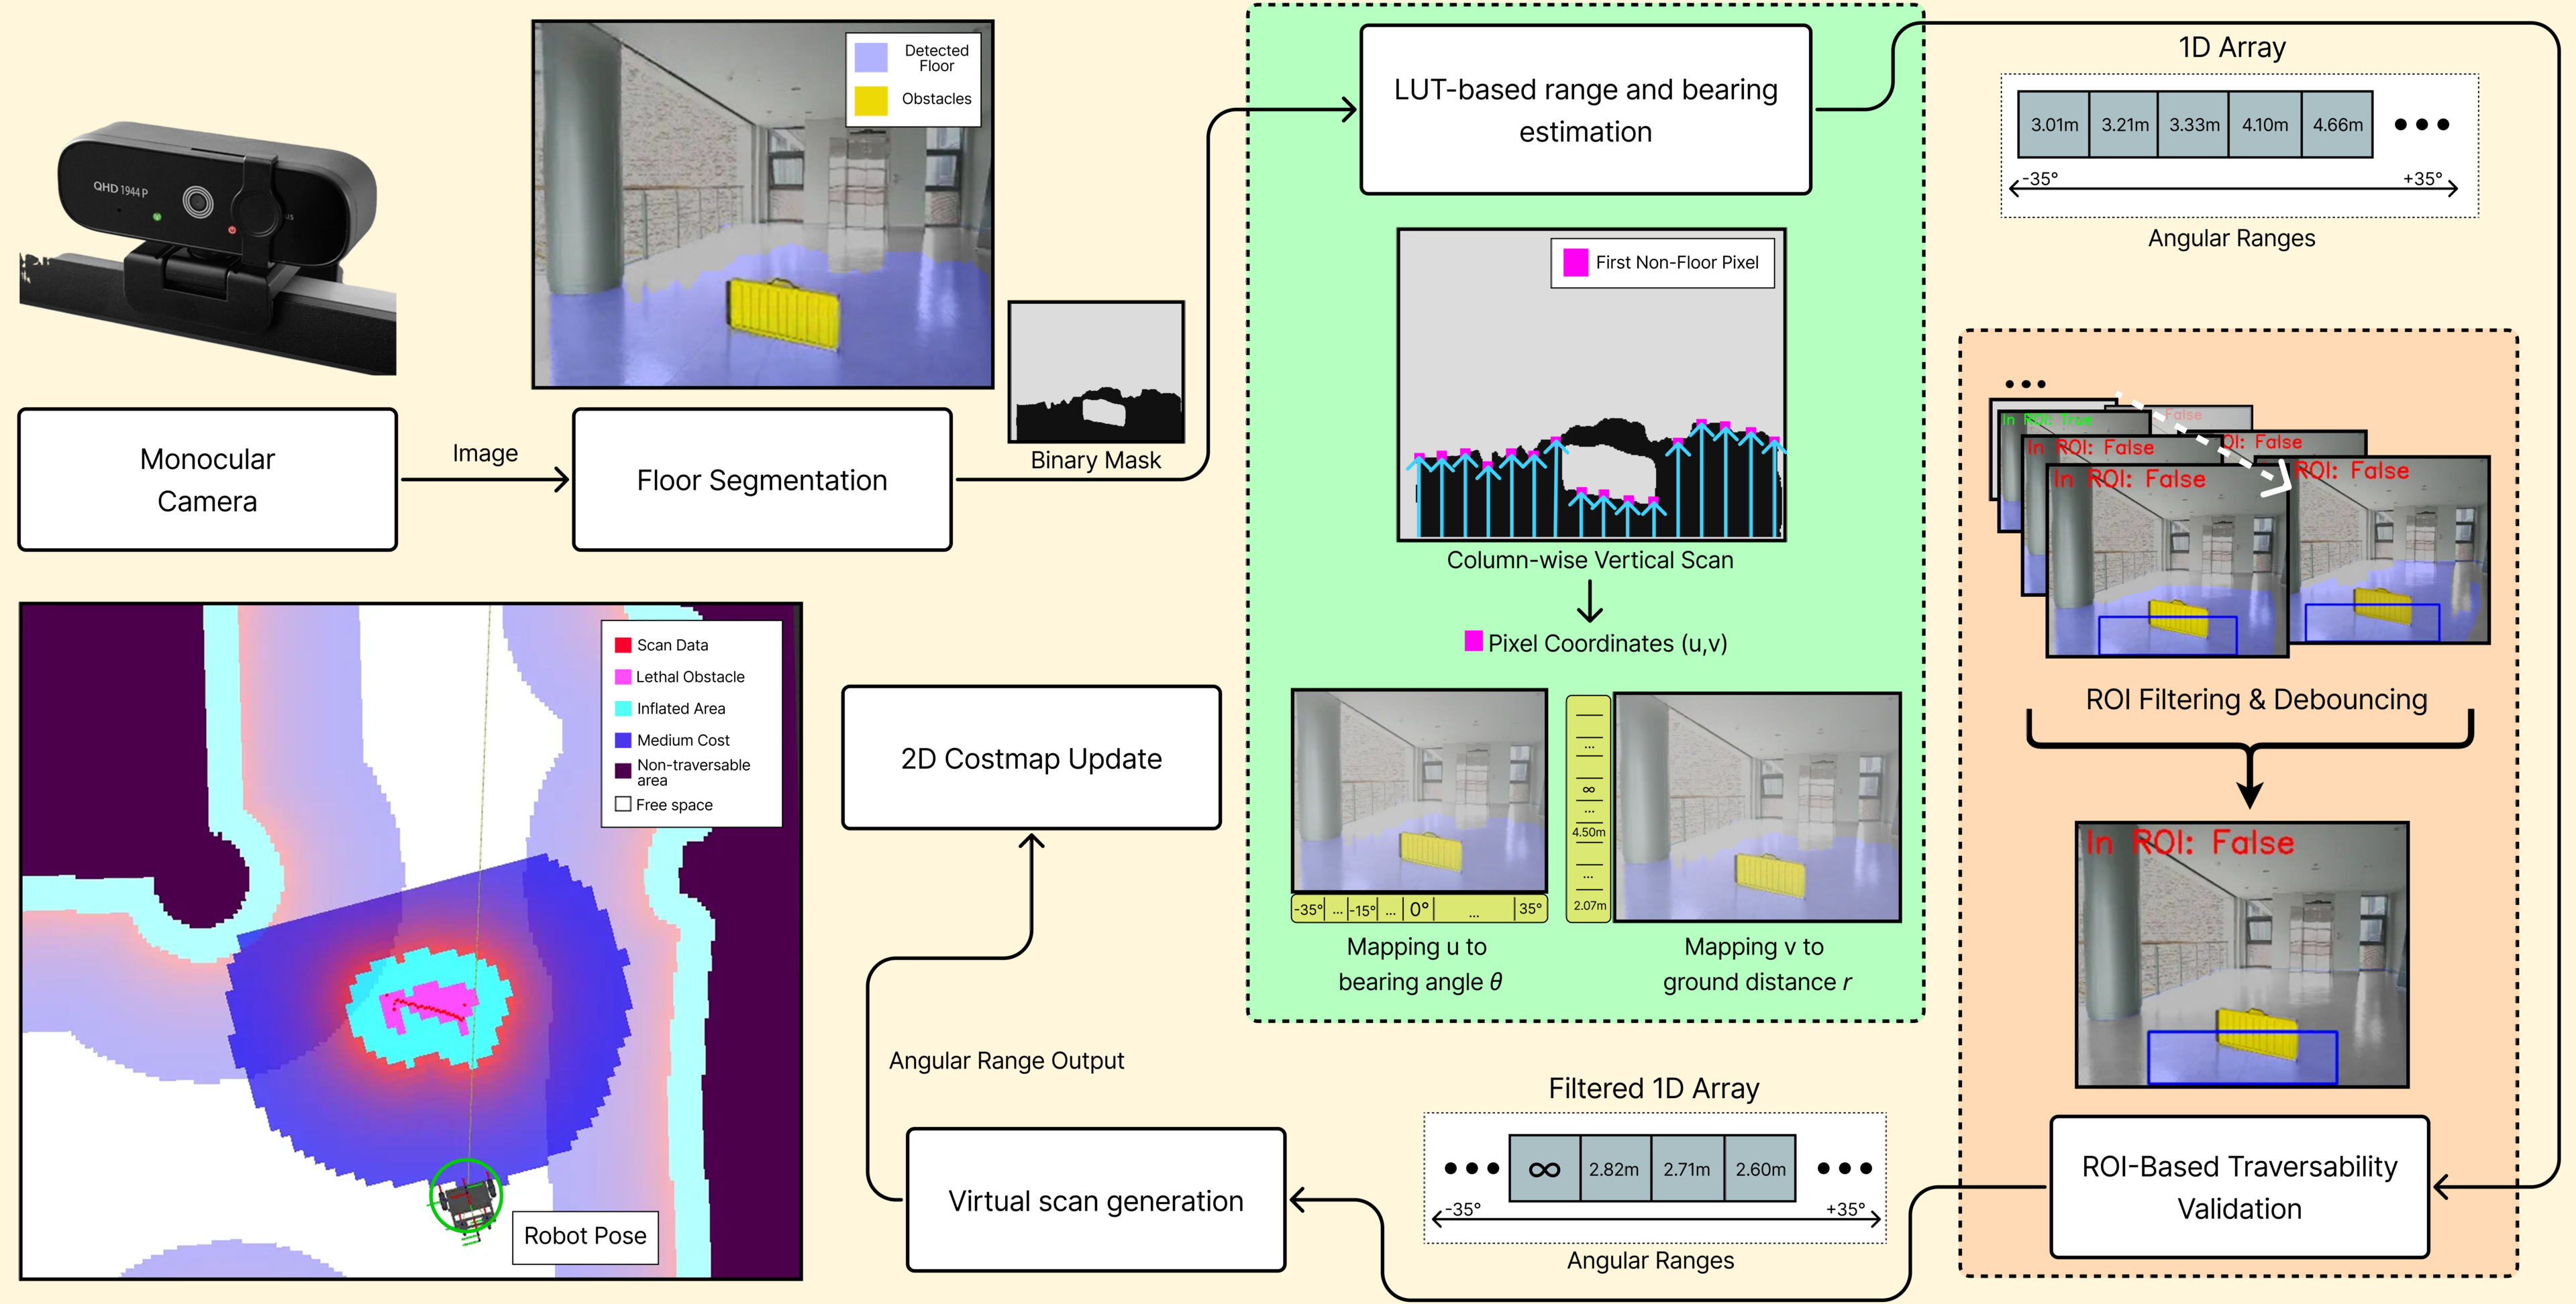
\includegraphics[width=0.95\textwidth]{pipeline}
\caption{Overview of the proposed virtual-scan pipeline, illustrating the full processing flow.}
\label{fig:pipeline}
\end{figure*}

\subsection{Floor Segmentation}\label{sec:floorseg}

Floor segmentation distinguishes traversable ground from potential obstacles and provides the binary mask used by the downstream LUT and ROI modules. We use YOLOv11n-seg, a nano-size instance-segmentation model from the Ultralytics YOLO11 family~\cite{ultralytics_2024_ultralytics}. Incoming frames are resized uniformly and processed at fixed intervals through a ROS 2 timer callback. The model is fine-tuned with supervised annotations for a dedicated floor class using manually annotated indoor floor images.

The model outputs a binary mask
\[
  M_{\mathrm{seg}} \in \{0,1\}^{H \times W},
\]
where
\[
  M_{\mathrm{seg}}[v,u] =
  \begin{cases}
    1, & \text{if pixel $(v,u)$ is classified as floor},\\
    0, & \text{if pixel $(v,u)$ is classified as non-floor}.
  \end{cases}
\]

Pixels with $M_{\mathrm{seg}}[v,u] = 1$ are treated as traversable, while $M_{\mathrm{seg}}[v,u] = 0$ indicates potential obstacles. The mask is forwarded to LUT-based range estimation (Section~\ref{sec:lut}) and ROI-based obstacle detection (Section~\ref{sec:roi}).

\subsection{LUT-Based Range and Bearing Estimation}\label{sec:lut}

To convert non-floor pixels into obstacle measurements in real time, we precompute two one-dimensional lookup tables (LUTs) offline. These tables encode the geometric relation between image coordinates and world-frame directions/distances, avoiding per-pixel trigonometric calls online.

\smallskip
\noindent\textbf{Camera Geometry.}
We assume a pinhole camera model with resolution $W\times H$, focal lengths $f_x,f_y$, and principal point $(c_x,c_y)$. A pixel $(u,v)$ corresponds to a camera-frame ray with horizontal bearing $\theta$ and vertical image angle $\phi$:
\begin{align*}
  \theta(u) &= \arctan\!\bigl((u - c_x)/f_x\bigr), \\
  \phi(v)   &= \arctan\!\bigl((v - c_y)/f_y\bigr).
\end{align*}
The camera is mounted at height $h$ and tilted downward by $\gamma$. The projection assumes a locally flat floor and fixed camera pose; if either changes, the LUTs must be recalibrated. With $\alpha(v)=\phi(v)+\gamma$, a ray intersects the ground at
\[
  d(v) \;=\; \frac{h}{\tan\!\bigl(\alpha(v)\bigr)}.
\]
for $\alpha(v)>0$; otherwise, we set $d(v)=\infty$.

\smallskip
\noindent\textbf{Lookup Table Construction.}
Using these relations, we build:
\begin{itemize}
  \item \textbf{Column-to-Bin LUT}
    \[
      L_{\mathrm{bin}}[u]
      = q\!\left(\theta(u)\right),
      \quad u = 0,\dots,W-1.
    \]
    Here, $q(\cdot)$ quantizes a horizontal bearing into one of the $N_{\mathrm{ang}}$ scan bins.
  \item \textbf{Row-to-Range LUT}
    \[
      L_{\mathrm{range}}[v]
      = \begin{cases}
        \displaystyle \frac{h}{\tan\!\bigl(\phi(v)+\gamma\bigr)}, & \phi(v)+\gamma>0,\\
        \infty, & \text{otherwise},
      \end{cases}
    \]
    for $v = 0,\dots,H-1$.
\end{itemize}
During virtual scan generation, each non-floor pixel uses $L_{\mathrm{bin}}[u]$ and $L_{\mathrm{range}}[v]$ to obtain its angular bin and distance estimate with two array lookups.

\subsection{ROI-Based Traversability Validation}\label{sec:roi}

To reduce noise, traversability is validated only inside a frontal ROI. A frame is considered clear when the floor-pixel ratio in this ROI exceeds $\tau_{\mathrm{floor}}$; a temporal debounce filter confirms the state only after the condition persists over recent frames. This reduces sensitivity to isolated mask errors before scan generation and costmap clearing.

\subsection{Virtual Scan Generation Algorithm}\label{sec:virtualscan}

Given $M_{\mathrm{seg}}$, ROI bounds, and the two LUTs, the virtual scan is generated as follows.

\begin{center}
\fbox{%
\begin{minipage}{0.94\linewidth}
\footnotesize
\noindent\textbf{Algorithm 1. Virtual Scan Generation}

\smallskip
\noindent\begin{tabularx}{\linewidth}{@{}rX@{}}
\textbf{Input:} & $M_{\mathrm{seg}}$, $L_{\mathrm{range}}$, $L_{\mathrm{bin}}$, ROI bounds, $N_{\mathrm{ang}}$\\
\textbf{Output:} & Virtual scan $S[1,\ldots,N_{\mathrm{ang}}]$
\end{tabularx}

\smallskip
\noindent\begin{tabularx}{\linewidth}{@{}rX@{}}
1: & Set $S[i]\gets\infty$ for all $i=1,\ldots,N_{\mathrm{ang}}$.\\
2: & For each image column $u=u_{\min},\ldots,u_{\max}$:\\
3: & \quad $\mathcal{V}_u \gets \{v\mid v_{\min}\le v\le v_{\max},\ M_{\mathrm{seg}}[v,u]=0\}$.\\
4: & \quad If $\mathcal{V}_u\neq\emptyset$:\\
5: & \quad\quad $v^*\gets\max(\mathcal{V}_u)$.\\
6: & \quad\quad $i\gets L_{\mathrm{bin}}[u]$.\\
7: & \quad\quad $r\gets L_{\mathrm{range}}[v^*]$.\\
8: & \quad\quad $S[i]\gets\min(S[i],r)$.\\
9: & Return $S$.
\end{tabularx}
\end{minipage}}
\end{center}

The lowest non-floor pixel $v^*$ approximates the image location where the obstacle meets the floor. The populated 1D array is then published as a scan message, with each angular bin holding the nearest observed obstacle distance within the ROI.

\subsection{ROS 2 Integration and Obstacle Presence Detection}\label{sec:ros2int}

The virtual scan generator is implemented as a single ROS 2 node connected to Nav2. At 10 Hz, it publishes the virtual scan $S$ and a floor-clear signal indicating whether ROI floor coverage exceeds $\tau_{\mathrm{floor}}$. If this signal remains active for longer than $T_{\mathrm{clear}}$, the node calls the local and global costmap-clear services to remove stale obstacles.

\subsection{Parameter Configuration}\label{sec:params}

Table~\ref{tab:params} summarizes the fixed parameters used in our implementation.
\begin{table}[H]
  \centering
  \caption{Key parameters and their values.}
  \label{tab:params}
  \footnotesize
  \begin{tabularx}{\linewidth}{@{}p{0.36\linewidth}p{0.18\linewidth}X@{}}
    \toprule
    Parameter & Value & Description \\
    \midrule
    $T_{\mathrm{seg}}$ & 0.2\,s & Mask inference period \\
    $(u_{\min},u_{\max})$ & (60, 260) & ROI columns \\
    $(v_{\min},v_{\max})$ & (180, 255) & ROI rows \\
    $N_{\mathrm{ang}}$ & 141 bins & Angular bins \\
    $\tau_{\mathrm{floor}}$ & 0.95 & Clear-floor ratio \\
    $T_{\mathrm{clear}}$ & 15\,s & Costmap-clear delay \\
    \bottomrule
  \end{tabularx}
\end{table}
These settings were selected in preliminary indoor tests and used consistently in all experiments.

\section{EXPERIMENTS}\label{sec4}
\label{sec:experiments}

This section evaluates the proposed virtual scan system through two experiments: range estimation under controlled static conditions and SLAM-based obstacle avoidance in a 10-meter indoor corridor with one static frontal obstacle. The goal is not to claim general replacement of LiDAR-based navigation, but to assess whether the system can provide usable obstacle information in a constrained structured environment.

\subsection{Experiment 1: Quantitative Evaluation of Range Precision}
\label{sec:experiment1}

This experiment quantifies whether the virtual scan provides sufficiently stable range estimates for coarse path planning and reactive behavior. Although the proposed scan is not intended to match the centimeter-level fidelity of LiDAR, it should provide consistent obstacle-distance cues under controlled indoor conditions.

We tested obstacles at 2.50\,m from the camera and three bearings. Fig.~\ref{fig:experiment1_setup} shows the physical setup used for the controlled range-evaluation trials.

\begin{figure}[H]
  \centering
  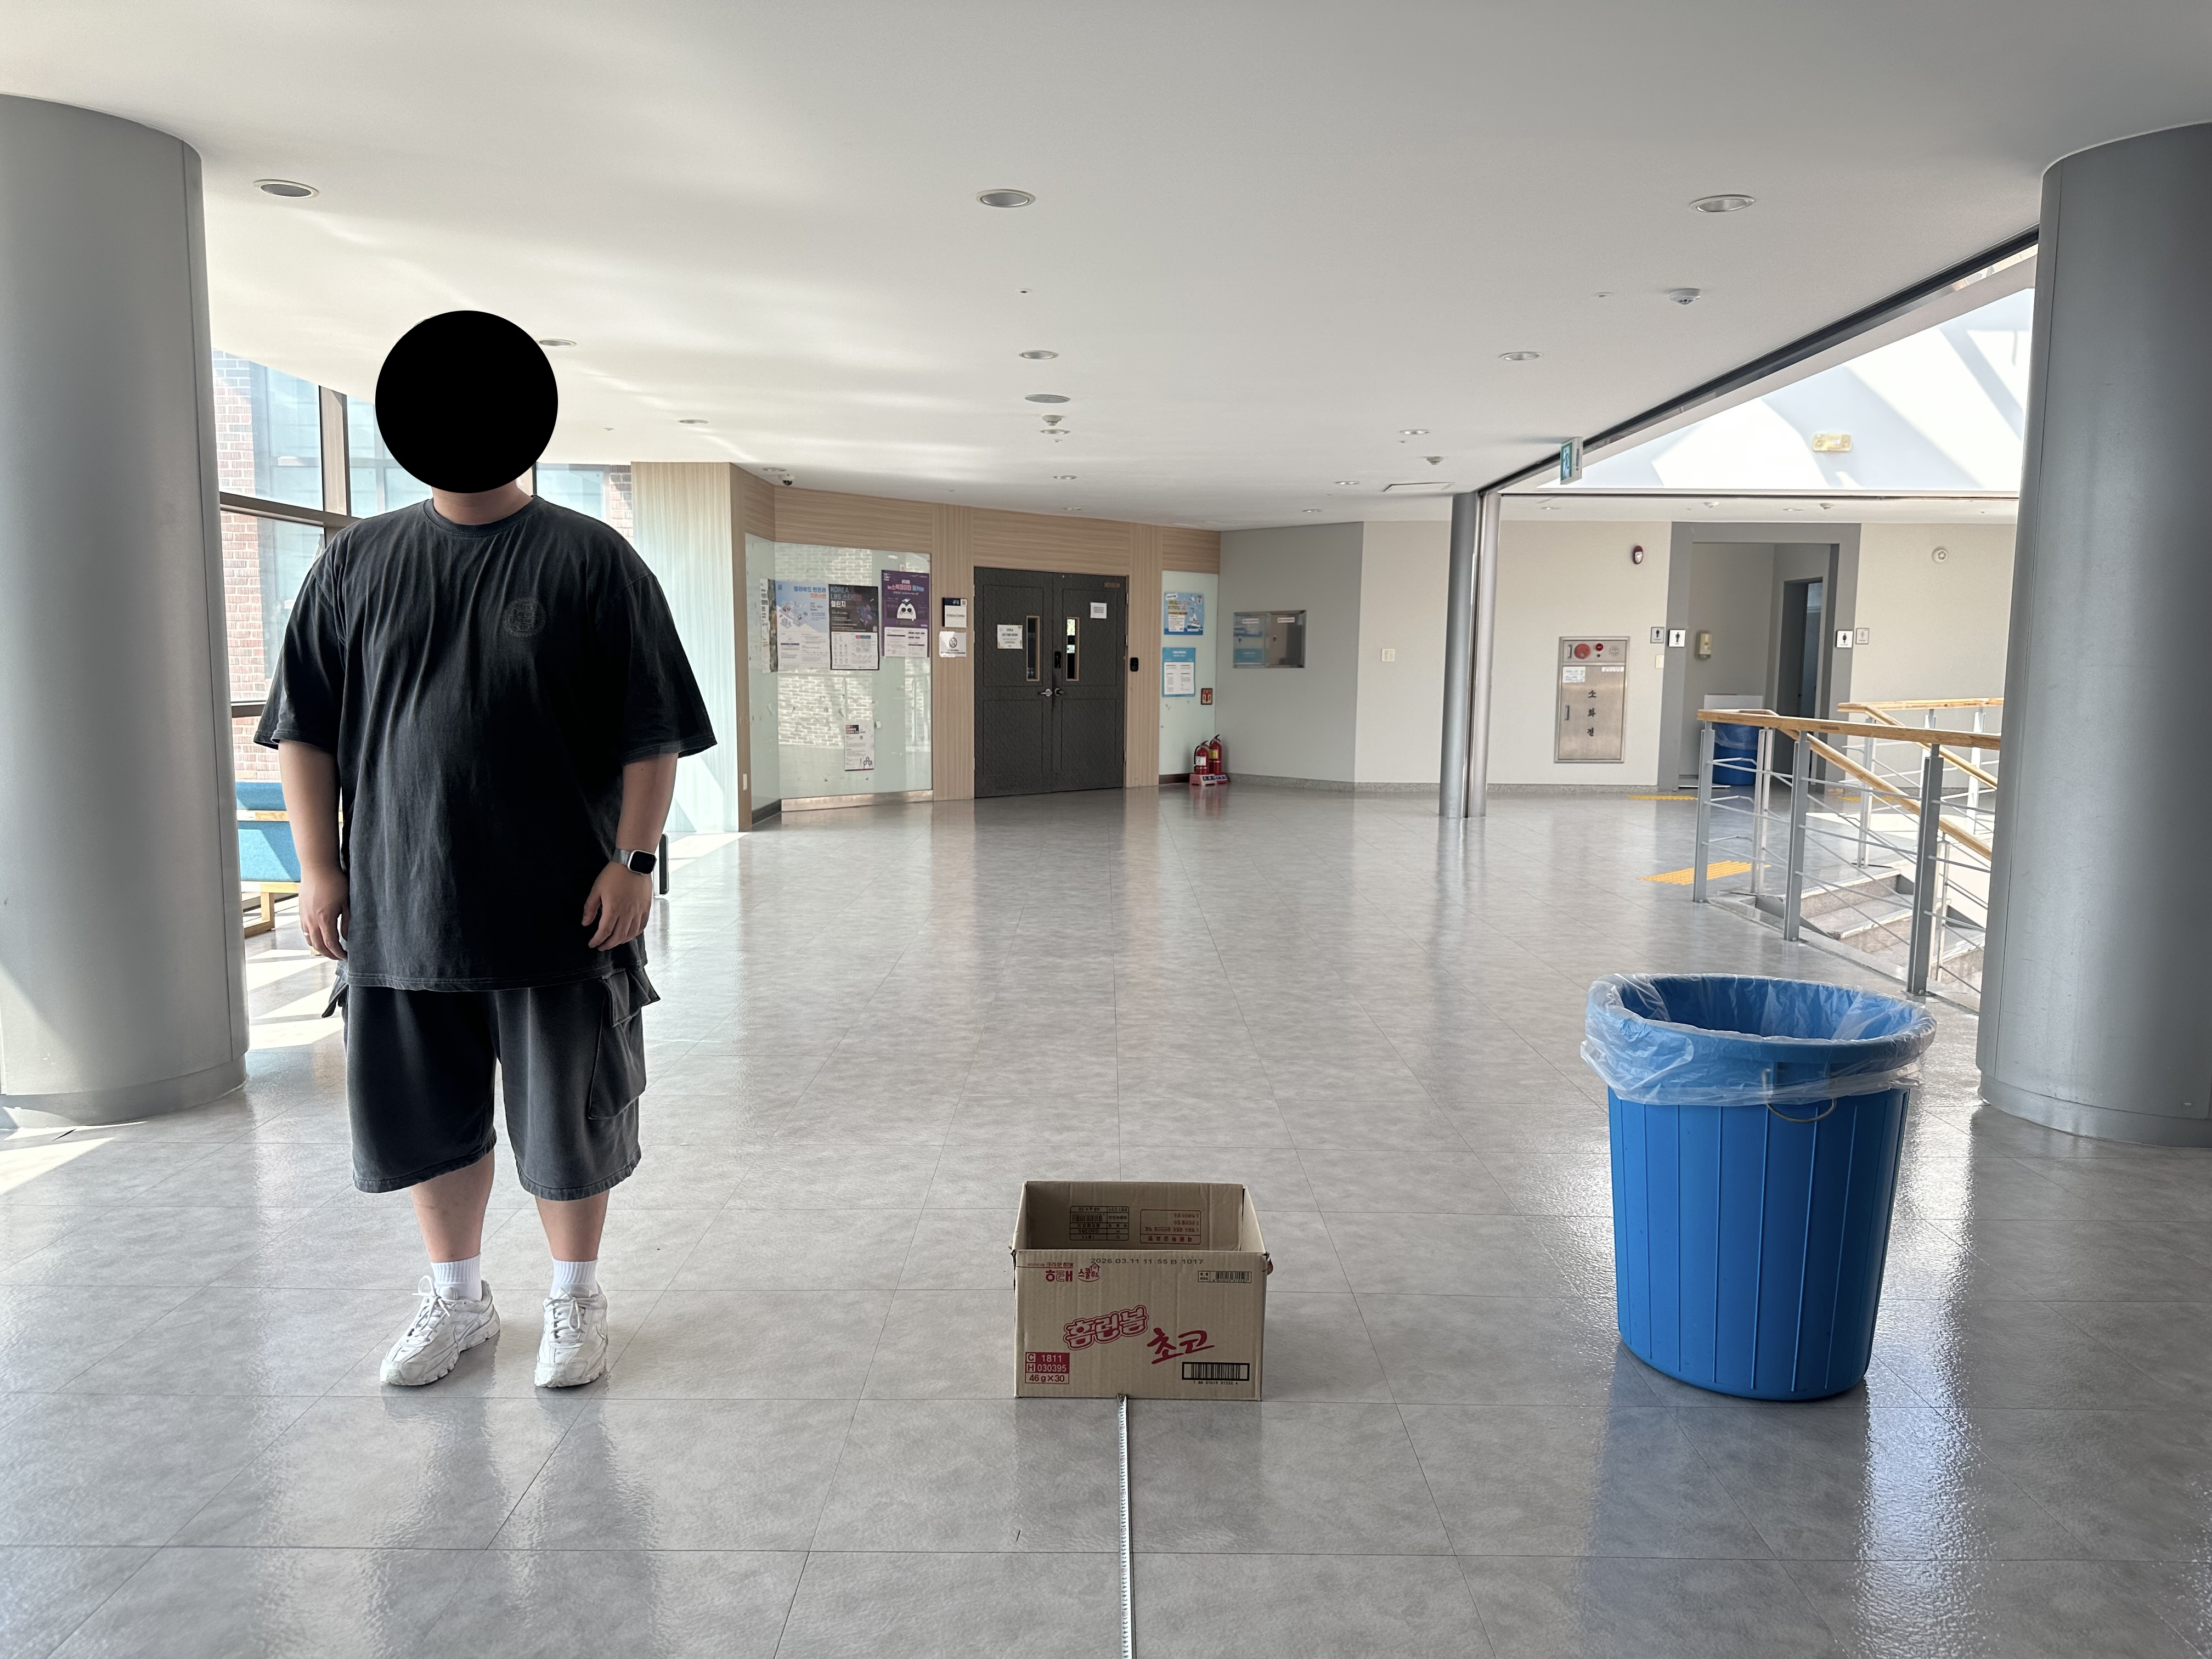
\includegraphics[width=0.9\linewidth]{experiment1_setup}
  \caption{Experiment 1 setup captured by the camera mounted on the parked robot. From left to right, the obstacles are a person at $+20^\circ$, a cardboard box at $0^\circ$, and a cylindrical trash can at $-20^\circ$.}
  \label{fig:experiment1_setup}
\end{figure}

\begin{itemize}
  \item \textbf{Front ($0^\circ$):} A cardboard box ($0.42\times0.335\times0.26$\,m) positioned directly in front.
  \item \textbf{Left ($+20^\circ$):} A standing adult male (1.78\,m tall).
  \item \textbf{Right ($-20^\circ$):} A cylindrical trash can ($0.63\times0.63\times0.75$\,m).
\end{itemize}

Ground truth distances were measured with a tape ($\pm1$\,cm), and angular positions were checked using a rotating stage and protractor ($\pm0.5^\circ$).

A total of 25 scan frames were collected for each condition over approximately 45 seconds. Fig.~\ref{fig:live_view} shows the live system view used during data collection.

\begin{figure}[H]
  \centering
  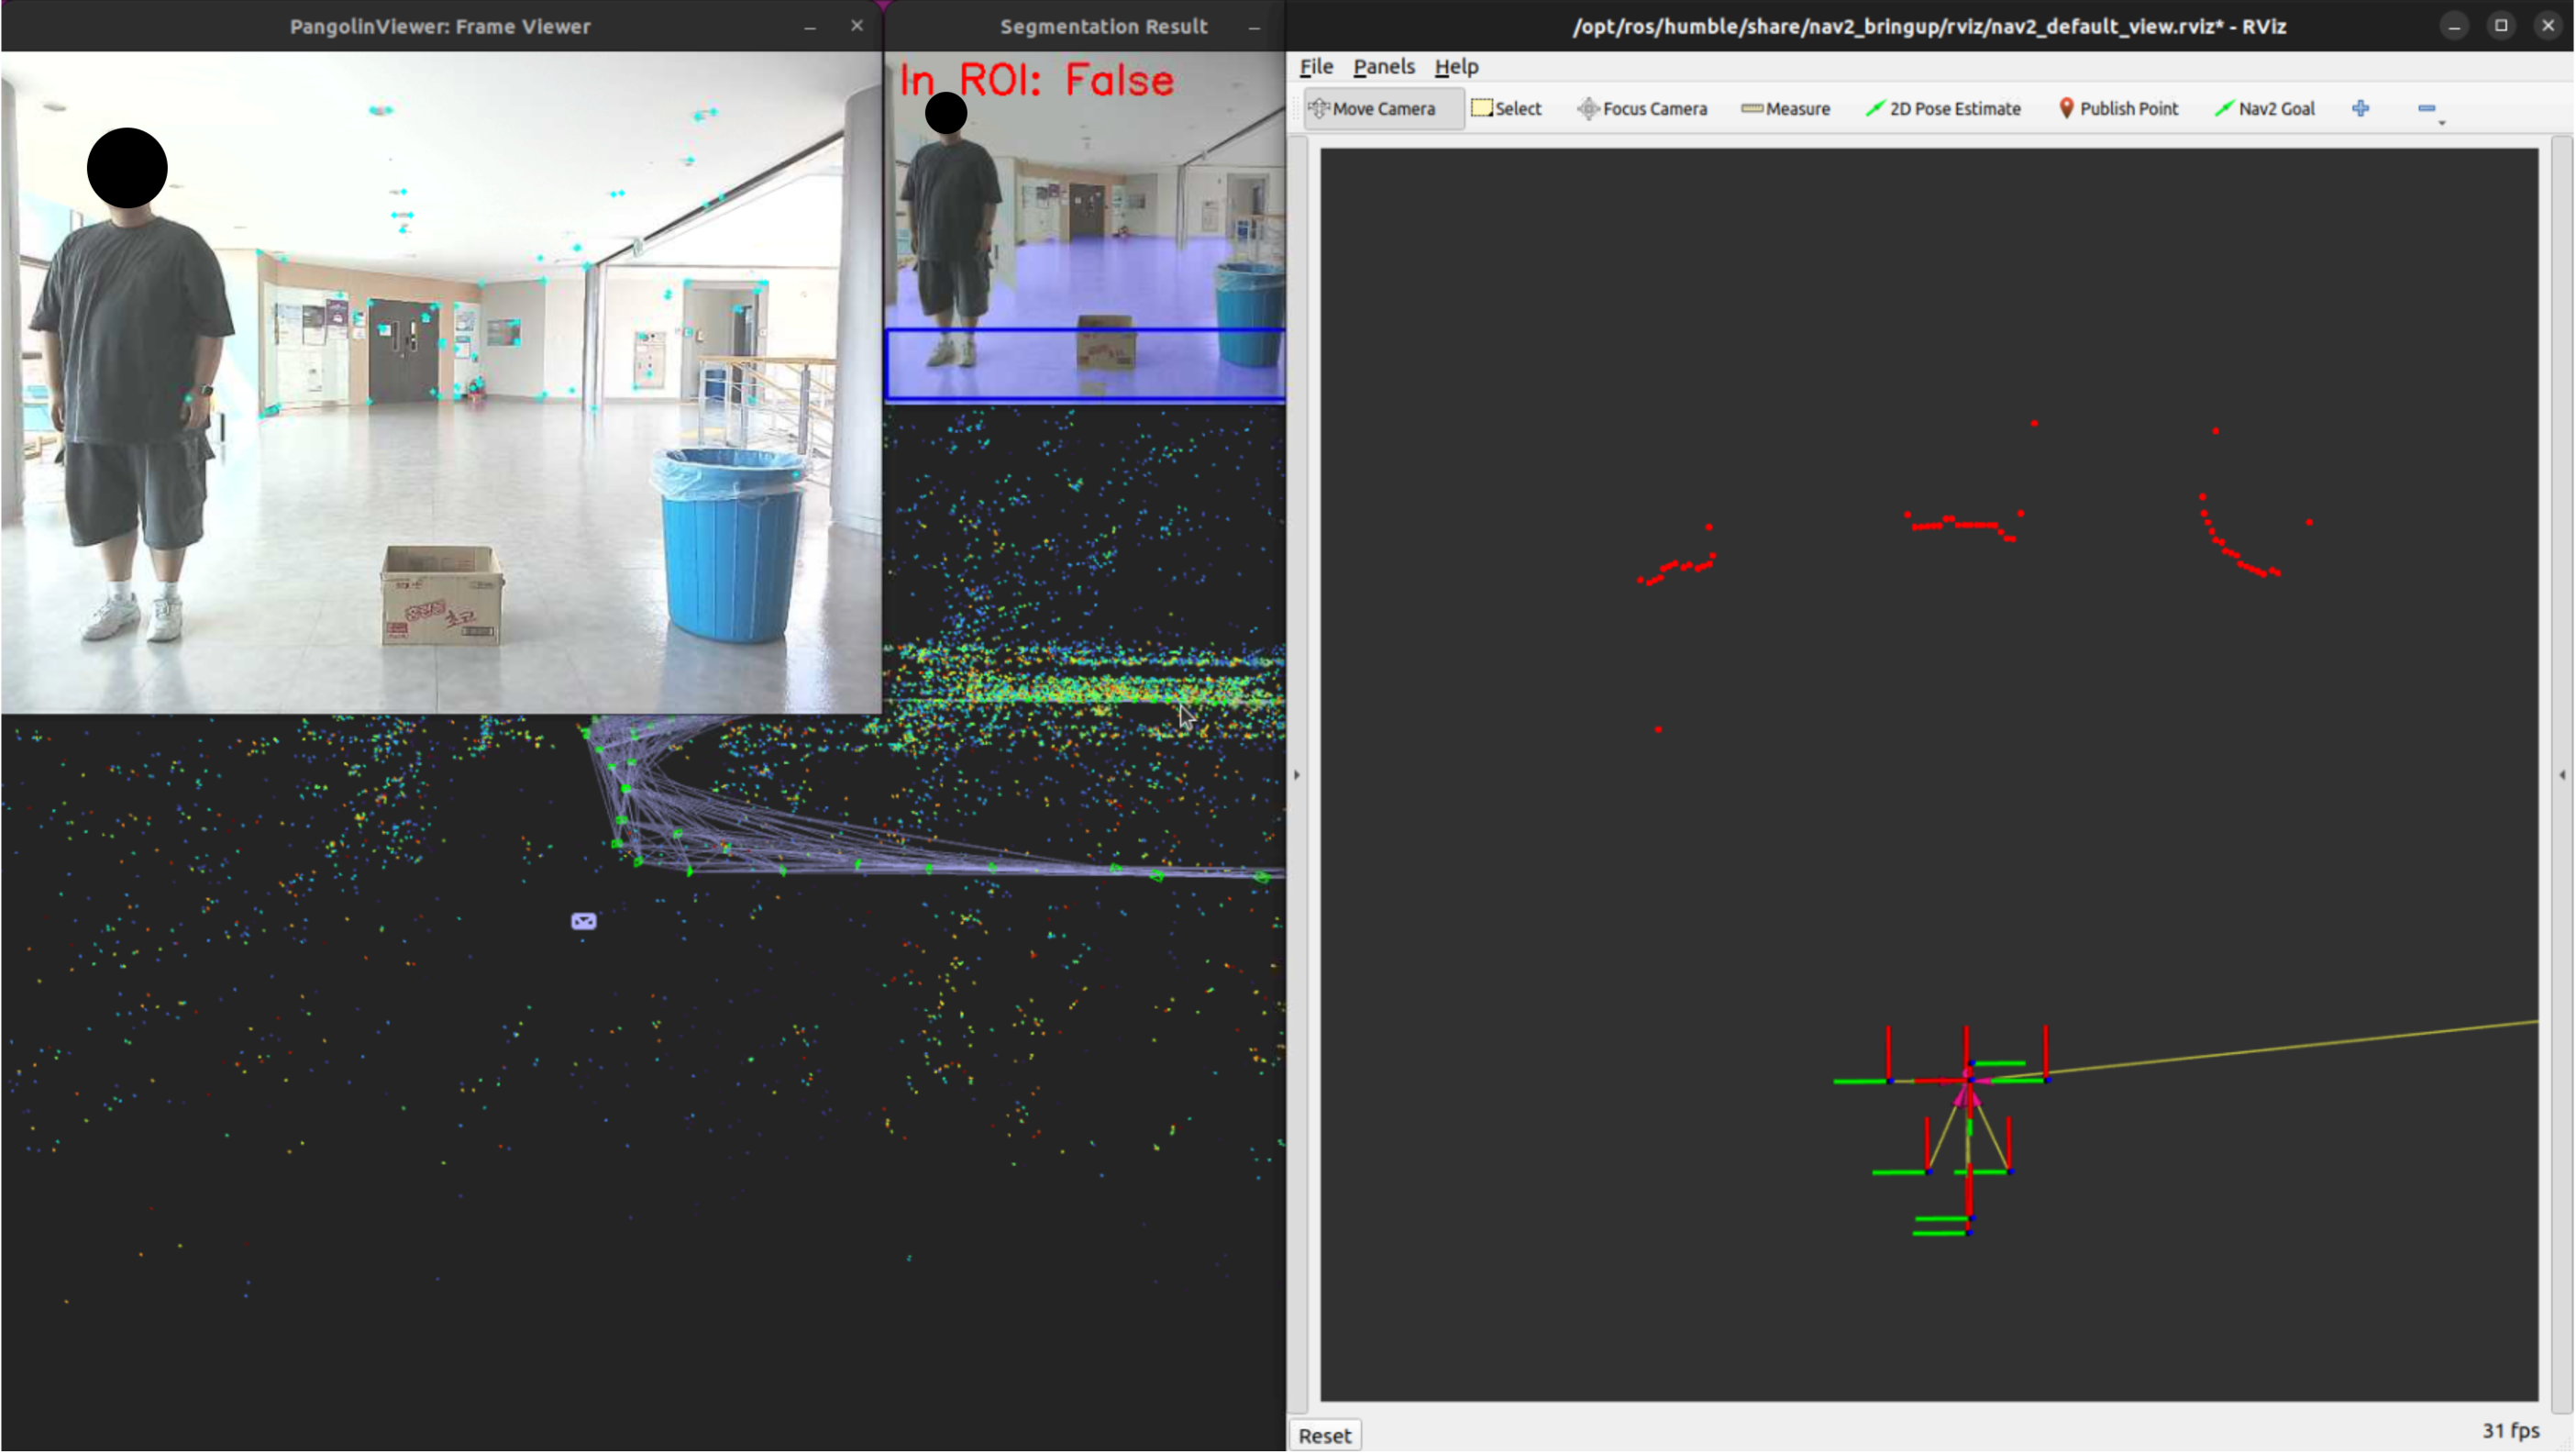
\includegraphics[width=0.9\linewidth]{live_view}
  \caption{Live view from our system's computer. The upper-center panel shows the segmentation status of the current frame, and the right panel visualizes the generated LaserScan.}
  \label{fig:live_view}
\end{figure}

\noindent\textbf{Results:}

Fig.~\ref{fig:experiment1_results} shows the first 10 virtual-scan samples collected under each test condition, and Table~\ref{tab:experiment1} summarizes the mean distance estimates and standard deviations. In the noisy-floor frontal condition, the estimated distance was 2.239\,m for a 2.50\,m target, corresponding to a $-$0.261\,m error, with a standard deviation of 0.172\,m. After floor noise mitigation, the frontal estimate shifted to 2.718\,m, yielding a +0.218\,m error with a standard deviation of 0.008\,m. The lateral conditions produced smaller errors, with +0.083\,m at $+20^\circ$ and +0.163\,m at $-20^\circ$.

\begin{figure*}[!b]
  \centering
  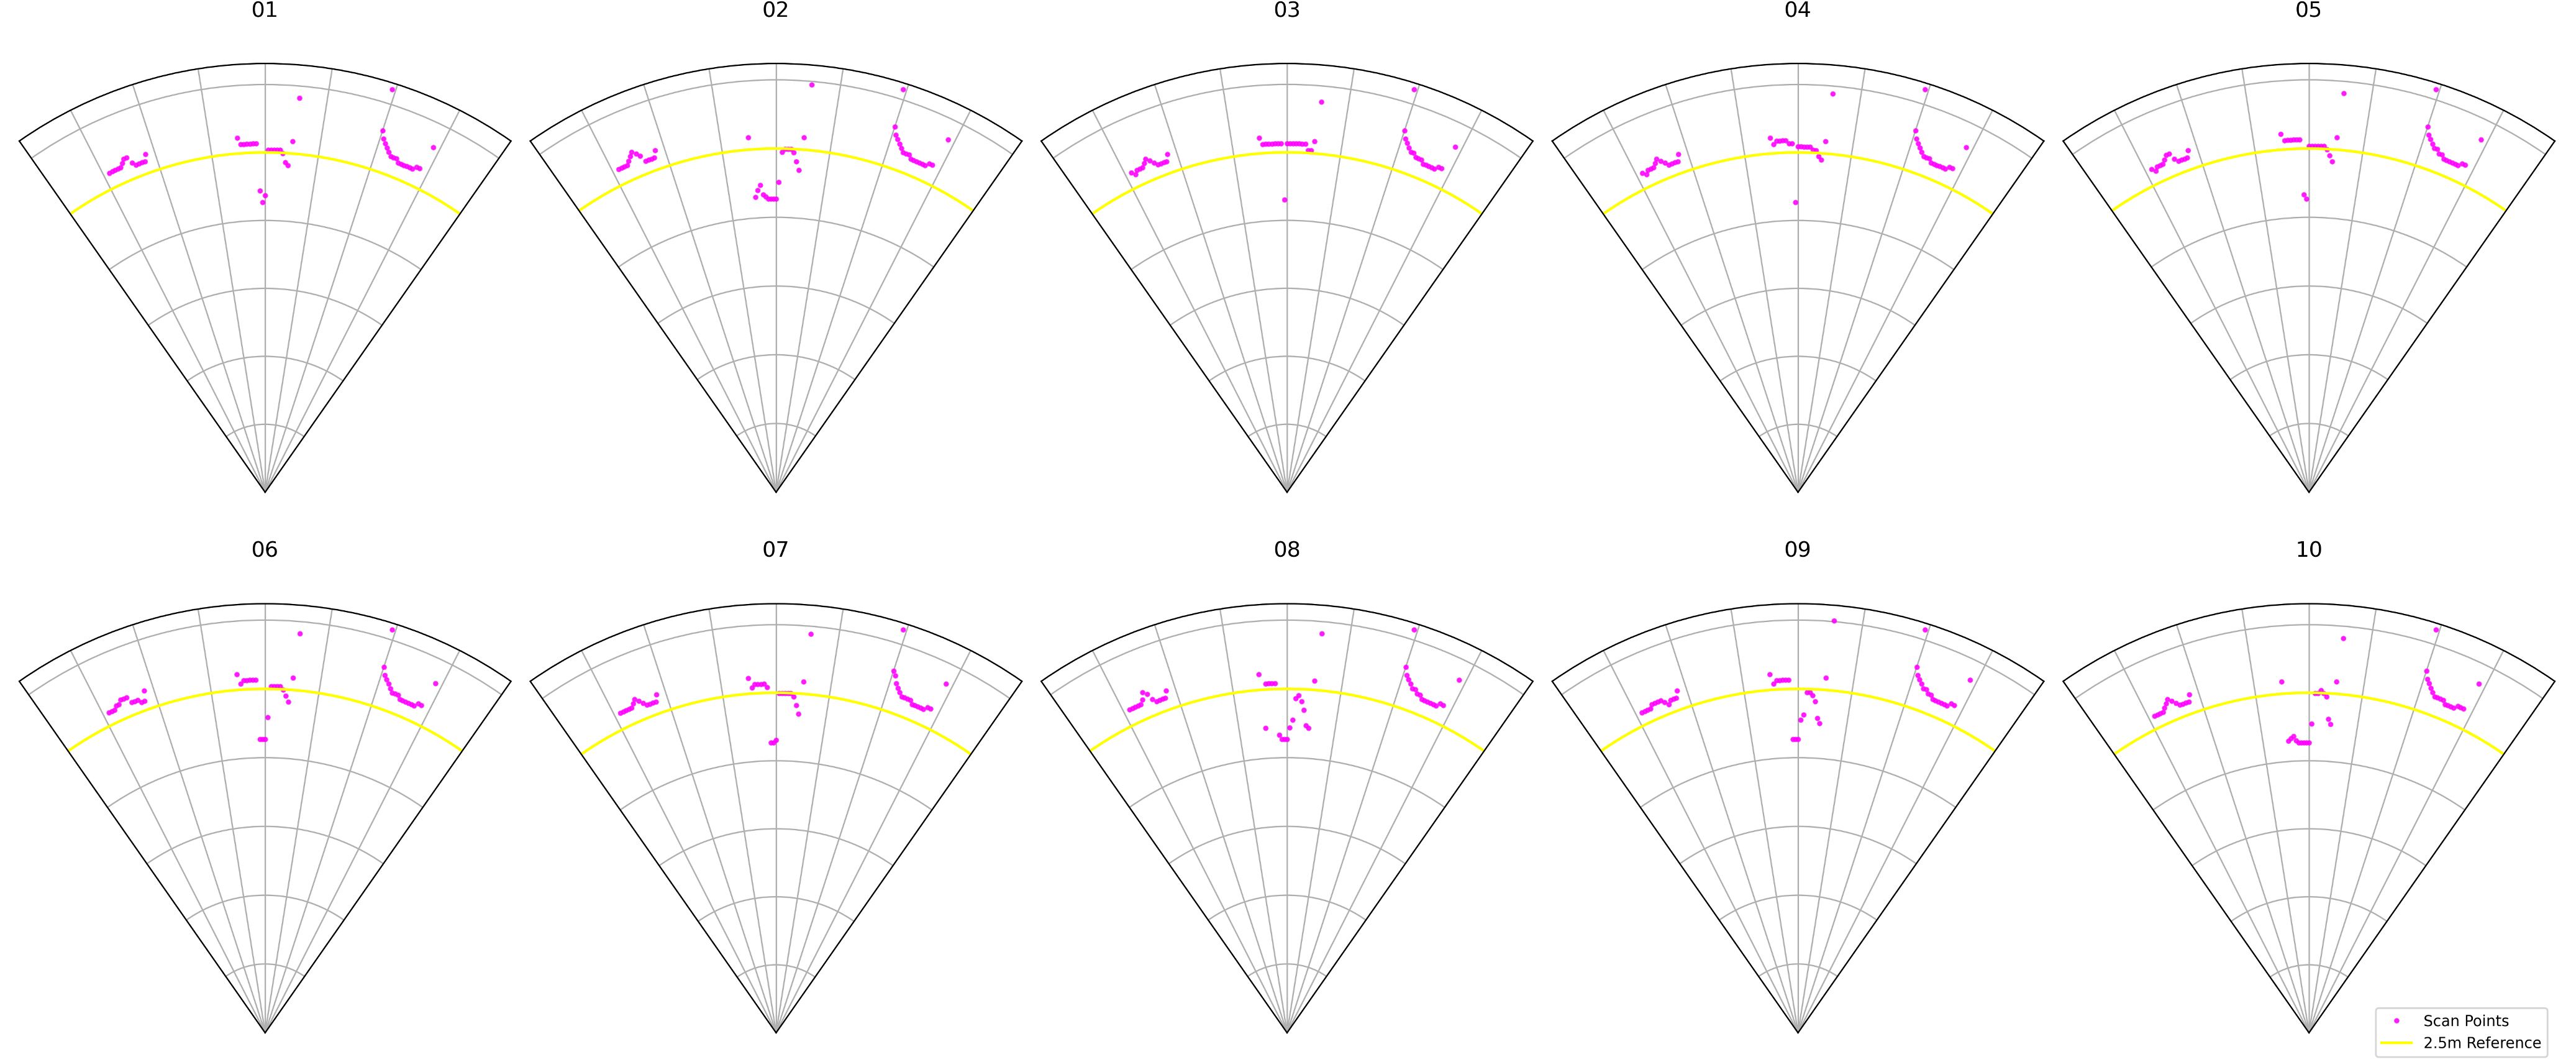
\includegraphics[width=0.86\textwidth]{experiment1_results}
  \caption{First 10 samples from Experiment 1. Magenta points denote virtual-scan points, and the reference line denotes the 2.5 m ground-truth distance.}
  \label{fig:experiment1_results}
\end{figure*}

\begin{table*}[!b]
  \centering
  \caption{Experiment 1 result.}
  \label{tab:experiment1}
  \begin{tabular}{lccccc}
    \toprule
    Condition & $N$ & Mean Distance (m) & Std. Dev. (m) & Mean Error (m) & Error Rate (\%) \\
    \midrule
    Front ($0^\circ$), noisy floor & 25 & 2.239 & 0.172 & $-$0.261 & $-$10.44 \\
    Front ($0^\circ$), clean floor & 25 & 2.718 & 0.008 & +0.218 & +8.72 \\
    Left ($+20^\circ$)             & 25 & 2.583 & 0.011 & +0.083 & +3.32 \\
    Right ($-20^\circ$)            & 25 & 2.663 & 0.000 & +0.163 & +6.52 \\
    \multicolumn{6}{p{0.92\textwidth}}{\footnotesize Note: The repeatable $-20^\circ$ result likely reflects strong trash-can/floor contrast and lower right-side glare.} \\
    \bottomrule
  \end{tabular}
\end{table*}

\subsection{Experiment 2: Static Obstacle Avoidance in SLAM}
\label{sec:experiment2}

This experiment assesses whether the proposed scan, integrated with SLAM and Nav2, can support obstacle avoidance in a structured indoor scenario. It uses only monocular vision, without active depth sensors such as LiDAR or stereo cameras.

\begin{itemize}
  \item \textbf{Robot Platform:} R1v2 from OMORobot.
  \item \textbf{Robot Computer:} NUC14RVK-B with Intel Core Ultra 7 155H CPU and 32\,GB RAM.
  \item \textbf{Camera:} LX-V11 monocular camera (5\,MP), facing forward.
  \item \textbf{SLAM Framework:} Stella VSLAM, based on OpenVSLAM.
  \item \textbf{Navigation Stack:} ROS 2 Nav2, using our virtual scan data to populate the local costmap.
\end{itemize}

The test was conducted along a 10-meter indoor corridor with a glossy floor and dynamic illumination from windows and ceiling lights. A single static obstacle was placed in front of the robot to evaluate forward obstacle avoidance. Fig.~\ref{fig:experiment2_setup} shows the experiment environment and obstacle placement.

\begin{figure}[H]
  \centering
  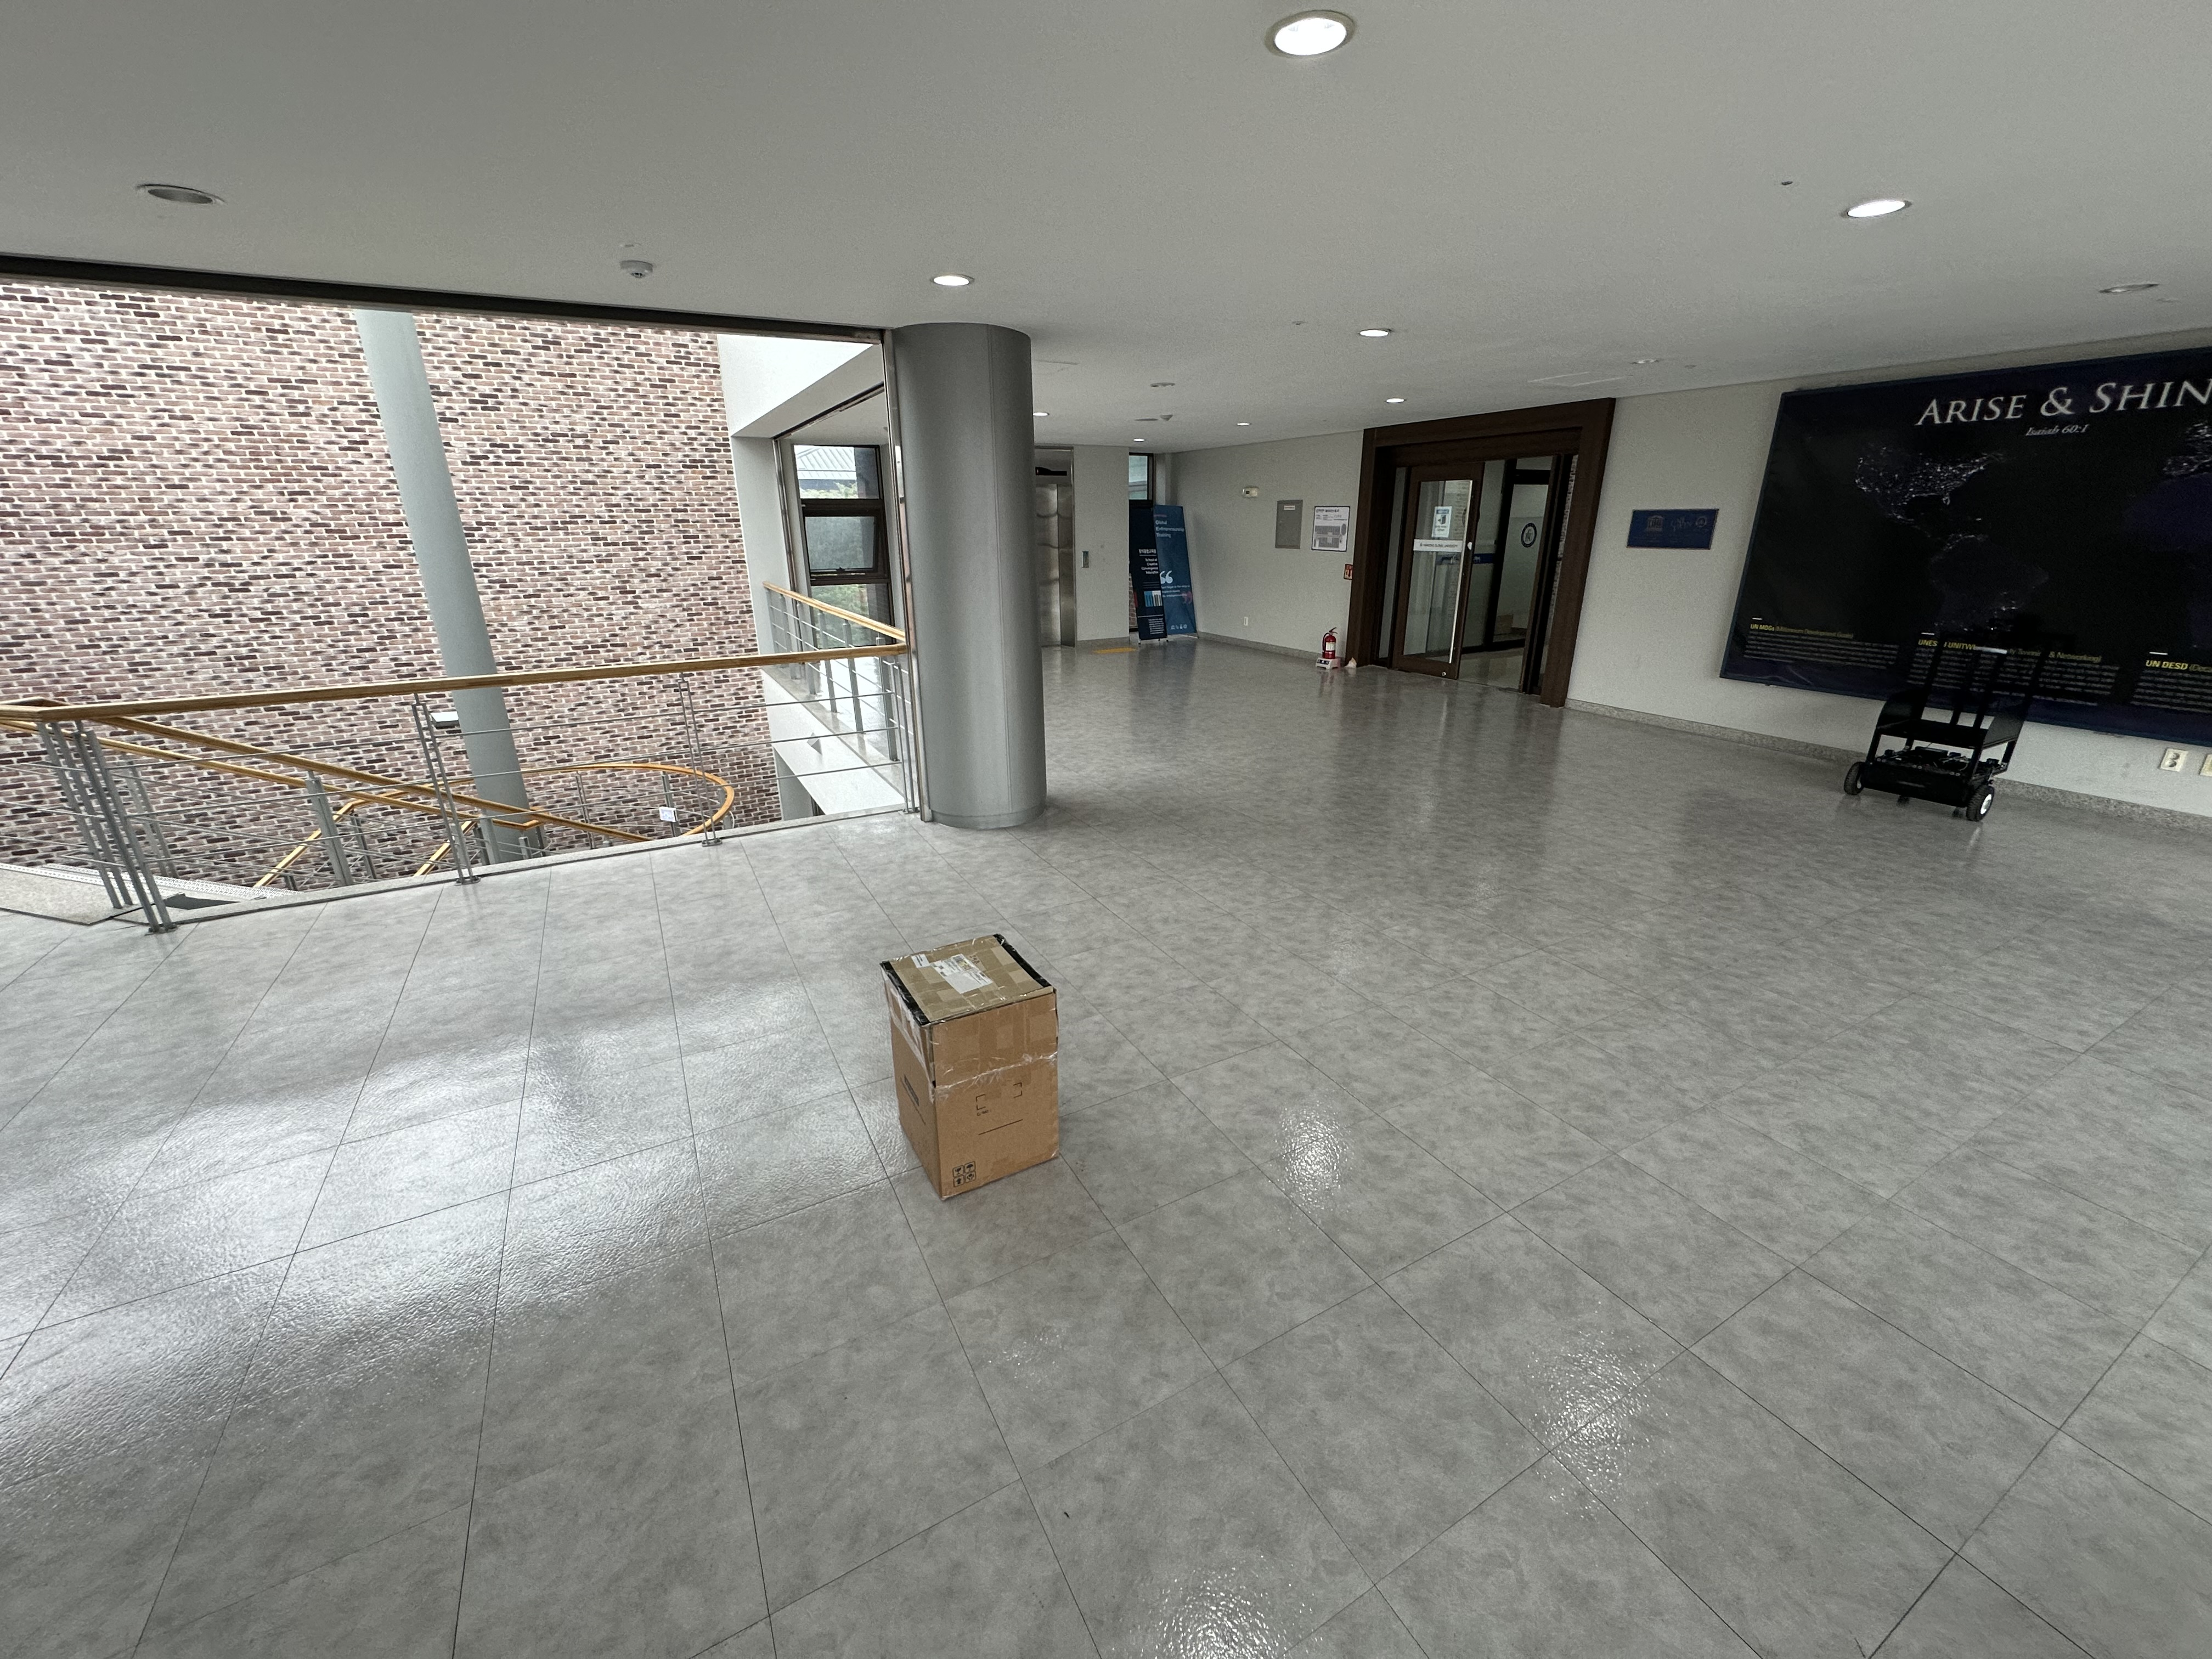
\includegraphics[width=0.9\linewidth]{experiment2_setup}
  \caption{Experiment 2 setup. The robot is located on the right side of the image, and the cardboard box is placed at the center of the robot's straight driving path.}
  \label{fig:experiment2_setup}
\end{figure}

\begin{itemize}
  \item A 10-meter straight navigation path
  \item One rectangular cardboard-box obstacle ($40\times40\times50$\,cm) positioned at the center of the straight path
  \item Variable lighting from windows and ceiling lights
\end{itemize}

For each trial, the robot planned toward a predefined goal using only the virtual scan and wheel-encoder odometry. Localization used the monocular SLAM front end, with no external IMU.

\noindent\textbf{Results:}

The robot completed 39 of 50 trials, corresponding to a 78\% success rate. This result demonstrates the feasibility of the proposed monocular virtual scan approach under constrained indoor conditions, but also highlights the need for improved robustness before practical deployment. During successful trials, obstacle cues were generated online and fed to Nav2, showing that the proposed scan can support obstacle avoidance in this controlled scenario. Among the 11 failed trials, eight were attributed to segmentation-induced obstacle jitter, and three occurred when the robot returned to the nominal path too quickly after avoidance.

Fig.~\ref{fig:nav2_obstacle_avoidance} shows a representative run: the frontal obstacle is detected from the camera view, represented in the local costmap, and avoided by the generated path.

\begin{figure*}[!b]
  \centering
  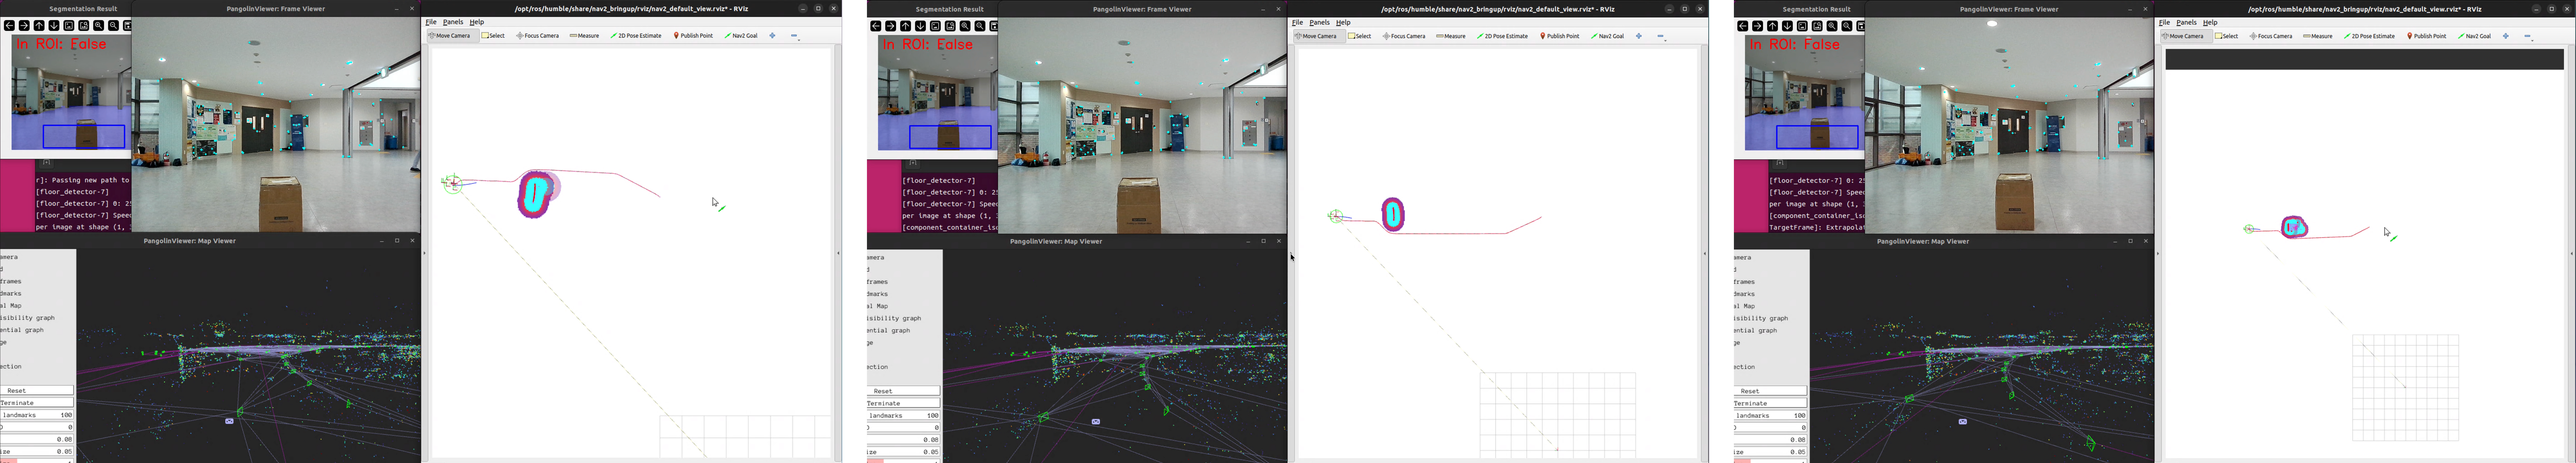
\includegraphics[width=0.88\textwidth]{nav2_obstacle_avoidance_sequence}
  \caption{Representative Nav2 integration sequence for the static frontal obstacle avoidance experiment. The three screenshots show the obstacle detected from the camera view and represented in the local costmap as the navigation stack generates an avoidance path.}
  \label{fig:nav2_obstacle_avoidance}
\end{figure*}

\subsection{Overall Discussion}
\label{sec:overall_discussion}

The two experiments jointly show that monocular virtual scanning can provide coarse but limited obstacle information for structured indoor navigation. Experiment 1 indicates that the scan does not provide LiDAR-level precision, but its error range is suitable for coarse proximity cues. Experiment 2 then shows that these cues can be generated online, represented in the Nav2 local costmap, and used to produce an avoidance path in a controlled static-obstacle scenario.

The 78\% success rate demonstrates the feasibility of the proposed monocular virtual scan approach under constrained indoor conditions, but also highlights the need for improved robustness before practical deployment. The dominant failure mode was segmentation-induced obstacle jitter. Fig.~\ref{fig:seg_artifact} shows a representative artifact observed under reflective floor conditions; such artifacts can shift the estimated obstacle position between frames and make local planning unstable. The remaining failures occurred when the robot returned to the nominal path too quickly after avoidance.

\begin{figure}[H]
  \centering
  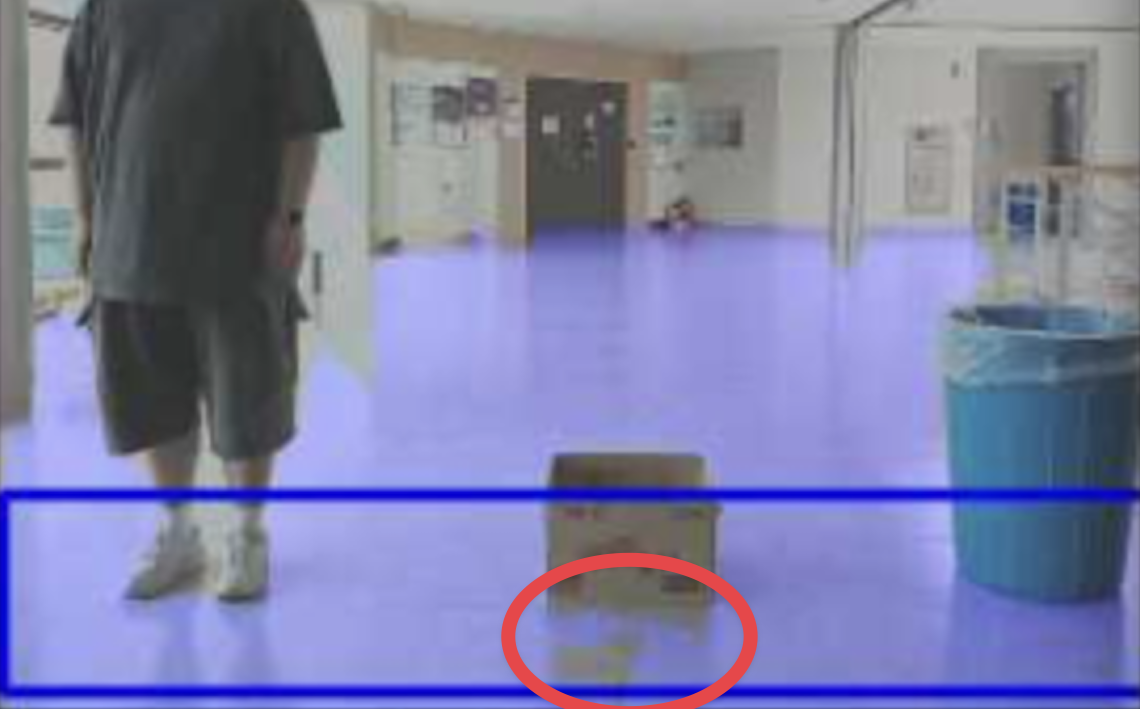
\includegraphics[width=0.9\linewidth]{segmentation_artifact}
  \caption{Example of a segmentation artifact. The red circle marks partial segmentation that can produce overly close distance estimates and obstacle jitter. This example illustrates a typical failure mode of the proposed system, where segmentation inconsistency causes unstable obstacle localization and may result in incorrect costmap updates.}
  \label{fig:seg_artifact}
\end{figure}

The failures should also be interpreted in light of the glossy floor, dynamic illumination, and imperfect match between the fine-tuning data and the campus test environment. Better target-domain data and stronger temporal filtering are expected to improve floor-mask consistency and obstacle avoidance.

Challenges remain for shadows, floor clutter, and highly reflective materials, but the results support further investigation of monocular scan generation as a lightweight sensing option for structured indoor AMR scenarios.

The present study should therefore be interpreted as a proof-of-concept evaluation rather than a comprehensive validation of monocular navigation.

\section{CONCLUSION}\label{sec5}

This paper presented a monocular virtual scan generation method for indoor mobile robot navigation. The system converts floor-segmentation results into a laser-scan-like representation using a lightweight YOLOv11n-seg floor detector, precomputed range/bearing LUTs, ROI-based validation, and ROS 2/Nav2 integration.

The generated scan provided coarse obstacle-distance cues that were sufficient for limited obstacle avoidance in the evaluated indoor scenario. In range estimation, the absolute error remained within 0.261\,m under static conditions, suitable for coarse obstacle awareness rather than precise ranging. In static frontal obstacle avoidance, the robot completed 39 of 50 trials over a 10-meter path with one cardboard-box obstacle, corresponding to a 78\% success rate. The Nav2 results confirm that the scan can be represented in the local costmap and used to produce an avoidance path in this constrained scenario.

The main limitations are floor-segmentation stability and post-avoidance path recovery. Future work will adapt the segmentation dataset to target environments, increase data diversity, apply temporal filtering, and evaluate diverse environments, dynamic obstacles, and longer routes.

The proposed approach relies on several assumptions, including a locally planar floor, a fixed camera pose, and sufficiently accurate floor segmentation. Its performance may degrade under reflective surfaces, severe illumination changes, transparent obstacles, or environments significantly different from the training data. Therefore, the method should currently be viewed as a lightweight supplementary sensing strategy rather than a replacement for dedicated range sensors.


\section*{ACKNOWLEDGEMENTS}
This research was supported by the ANCHOR program Glocal University 30 through the Gyeongbuk ANCHOR CENTER, funded by the Ministry of Education (MOE) and the Gyeongsangbuk-do, Republic of Korea. (2026-ANCHOR-15-119)


\section*{DECLARATIONS}

\subsection*{Conflict of Interest}
The authors declare no competing interests.

\subsection*{Authors' Contributions}
Hyunseo Lee, Gunmin Yoo, and Hyunwoo Gu contributed equally to this work, including system implementation, experiments, analysis, and manuscript preparation. Sung Soo Hwang supervised the research, guided the methodology, and served as the corresponding author. All authors reviewed and approved the manuscript.

\subsection*{Data Availability}
The floor-segmentation fine-tuning dataset is publicly available at \url{https://universe.roboflow.com/projects-aw2cm/floor-segmentation-wesrg}. Additional experimental records and processed evaluation materials are available from the corresponding author upon reasonable request. The Virtual Scan Generator package for ROS 2 Humble is planned to be released upon publication.

\subsection*{Use of AI Tools}
ChatGPT by OpenAI and Codex by OpenAI were used to assist with \LaTeX{} editing and composition, translation, and grammar correction. All scientific content, experimental results, interpretations, references, and the final manuscript were reviewed and verified by the authors, who take full responsibility for the content of this work.



\begin{reference}
\bibitem{gvrnextgenerationtechnologiesresearchteam_2026_autonomous} GVR Next Generation Technologies Research Team, ``Autonomous mobile robots market size report, 2026--2033,'' Grand View Research, 2026. [Online]. Available: \url{https://www.grandviewresearch.com/industry-analysis/autonomous-mobile-robots-market}

\bibitem{liu_2024_a} \doi{Y. Liu, S. Wang, Y. Xie, T. Xiong, and M. Wu, ``A review of sensing technologies for indoor autonomous mobile robots,'' \textit{Sensors}, vol. 24, no. 4, Art. no. 1222, 2024.}{10.3390/s24041222}

\bibitem{yang_2019_semantic} \doi{F. Yang, L. Li, F. Su, D. Li, H. Zhu, S. Ying, X. Zuo, and L. Tang, ``Semantic decomposition and recognition of indoor spaces with structural constraints for 3D indoor modelling,'' \textit{Automation in Construction}, vol. 106, Art. no. 102913, 2019.}{10.1016/j.autcon.2019.102913}

\bibitem{deepthadamodaran_2023_experimental} \doi{D. Damodaran, S. Mozaffari, S. Alirezaee, and M. J. Ahamed, ``Experimental analysis of the behavior of mirror-like objects in LiDAR-based robot navigation,'' \textit{Applied Sciences}, vol. 13, no. 5, Art. no. 2908, 2023.}{10.3390/app13052908}

\bibitem{yang_2011_on} \doi{S.-W. Yang and C.-C. Wang, ``On solving mirror reflection in LIDAR sensing,'' \textit{IEEE/ASME Transactions on Mechatronics}, vol. 16, no. 2, pp. 255--265, 2011.}{10.1109/TMECH.2010.2040113}

\bibitem{tibebu_2021_lidarbased} \doi{H. Tibebu, J. Roche, V. De Silva, and A. Kondoz, ``LiDAR-based glass detection for improved occupancy grid mapping,'' \textit{Sensors}, vol. 21, no. 7, Art. no. 2263, 2021.}{10.3390/s21072263}

\bibitem{mei_2021_depthaware} \doi{H. Mei, B. Dong, W. Dong, P. Peers, X. Yang, Q. Zhang, and X. Wei, ``Depth-aware mirror segmentation,'' in \textit{Proc. IEEE/CVF Conf. Computer Vision and Pattern Recognition}, 2021, pp. 3043--3052.}{10.1109/cvpr46437.2021.00306}

\bibitem{sajjan_2020_clear} \doi{S. Sajjan, M. Moore, M. Pan, G. Nagaraja, J. Lee, A. Zeng, and S. Song, ``Clear Grasp: 3D shape estimation of transparent objects for manipulation,'' in \textit{Proc. IEEE Int. Conf. Robotics and Automation}, 2020, pp. 3634--3642.}{10.1109/ICRA40945.2020.9197518}

\bibitem{singh_2019_multidata} \doi{R. Singh and K. S. Nagla, ``Multi-data sensor fusion framework to detect transparent object for the efficient mobile robot mapping,'' \textit{International Journal of Intelligent Unmanned Systems}, vol. 7, no. 1, pp. 2--18, 2019.}{10.1108/ijius-05-2018-0013}

\bibitem{shariqfarooqbhat_2021_adabins} \doi{S. F. Bhat, I. Alhashim, and P. Wonka, ``AdaBins: Depth estimation using adaptive bins,'' in \textit{Proc. IEEE/CVF Conf. Computer Vision and Pattern Recognition}, 2021, pp. 4009--4018.}{10.1109/cvpr46437.2021.00400}

\bibitem{ranftl_2021_vision} \doi{R. Ranftl, A. Bochkovskiy, and V. Koltun, ``Vision transformers for dense prediction,'' in \textit{Proc. IEEE/CVF Int. Conf. Computer Vision}, 2021, pp. 12159--12168.}{10.1109/ICCV48922.2021.01196}

\bibitem{ultralytics_2024_ultralytics} Ultralytics, ``Ultralytics YOLO11,'' 2024. [Online]. Available: \url{https://docs.ultralytics.com/models/yolo11}

\bibitem{macenski_2022_robot} \doi{S. Macenski, T. Foote, B. Gerkey, C. Lalancette, and W. Woodall, ``Robot Operating System 2: Design, architecture, and uses in the wild,'' \textit{Science Robotics}, vol. 7, Art. no. eabm6074, 2022.}{10.1126/scirobotics.abm6074}

\bibitem{macenski_2020_the} \doi{S. Macenski, F. Martin, R. White, and J. G. Clavero, ``The Marathon 2: A navigation system,'' in \textit{Proc. IEEE/RSJ Int. Conf. Intelligent Robots and Systems}, 2020.}{10.1109/iros45743.2020.9341207}

\bibitem{openrobotics_sensor_msgslaserscan} Open Robotics, ``sensor\_msgs/LaserScan documentation.'' [Online]. Available: \url{https://docs.ros.org/en/noetic/api/sensor_msgs/html/msg/LaserScan.html}

\bibitem{opennavigationllc_2023_costmap} Open Navigation LLC, ``Costmap 2D--Nav2 1.0.0 documentation,'' 2023. [Online]. Available: \url{https://docs.nav2.org/configuration/packages/configuring-costmaps.html}

\bibitem{li_2020_lidar} \doi{Y. Li and J. Ibanez-Guzman, ``Lidar for autonomous driving: The principles, challenges, and trends for automotive lidar and perception systems,'' \textit{IEEE Signal Processing Magazine}, vol. 37, no. 4, pp. 50--61, 2020.}{10.1109/msp.2020.2973615}

\bibitem{yusuf_2022_iotbased} \doi{M. Yusuf, A. Zaidi, A. Haleem, S. Bahl, M. Javaid, S. B. Garg, and J. Garg, ``IoT-based low-cost 3D mapping using 2D Lidar for different materials,'' \textit{Materials Today: Proceedings}, vol. 57, Part 2, pp. 942--947, 2022.}{10.1016/j.matpr.2022.03.161}

\bibitem{wang_2017_detecting} \doi{X. Wang and J. Wang, ``Detecting glass in simultaneous localisation and mapping,'' \textit{Robotics and Autonomous Systems}, vol. 88, pp. 97--103, 2017.}{10.1016/j.robot.2016.11.003}

\bibitem{wang_2021_a} \doi{S. Wang, L. Wang, X. He, and Y. Cao, ``A monocular vision obstacle avoidance method applied to indoor tracking robot,'' \textit{Drones}, vol. 5, no. 4, Art. no. 105, 2021.}{10.3390/drones5040105}

\bibitem{dang_2023_obstacle} \doi{T.-V. Dang and N.-T. Bui, ``Obstacle avoidance strategy for mobile robot based on monocular camera,'' \textit{Electronics}, vol. 12, no. 8, Art. no. 1932, 2023.}{10.3390/electronics12081932}

\bibitem{openrobotics_2020_depthimage_to_laserscan} Open Robotics, ``depthimage\_to\_laserscan package documentation,'' 2020. [Online]. Available: \url{https://wiki.ros.org/depthimage_to_laserscan}

\bibitem{openrobotics_2015_pointcloud_to_laserscan} Open Robotics, ``pointcloud\_to\_laserscan package documentation,'' 2015. [Online]. Available: \url{https://wiki.ros.org/pointcloud_to_laserscan}

\bibitem{quigley_2009_ros} M. Quigley, K. Conley, B. Gerkey, J. Faust, T. Foote, J. Leibs, R. Wheeler, and A. Y. Ng, ``ROS: An open-source robot operating system,'' in \textit{Proc. ICRA Workshop on Open Source Software}, vol. 3, no. 3.2, 2009, p. 5.

\bibitem{macenski_2023_from} \doi{S. Macenski, T. Moore, D. V. Lu, A. Merzlyakov, and M. Ferguson, ``From the desks of ROS maintainers: A survey of modern \& capable mobile robotics algorithms in the Robot Operating System 2,'' \textit{Robotics and Autonomous Systems}, vol. 168, Art. no. 104493, 2023.}{10.1016/j.robot.2023.104493}

\bibitem{opennavigationllc_2025_denoise} Open Navigation LLC, ``Denoise layer parameters--Nav2 1.0.0 documentation,'' 2025. [Online]. Available: \url{https://docs.nav2.org/configuration/packages/costmap-plugins/denoise.html}

\bibitem{fox_1997_the} \doi{D. Fox, W. Burgard, and S. Thrun, ``The dynamic window approach to collision avoidance,'' \textit{IEEE Robotics \& Automation Magazine}, vol. 4, no. 1, pp. 23--33, 1997.}{10.1109/100.580977}

\bibitem{thrun_2010_probabilistic} S. Thrun, W. Burgard, and D. Fox, \textit{Probabilistic Robotics}. Cambridge, MA, USA: MIT Press, 2010.

\bibitem{elfes_1989_using} \doi{A. Elfes, ``Using occupancy grids for mobile robot perception and navigation,'' \textit{Computer}, vol. 22, no. 6, pp. 46--57, 1989.}{10.1109/2.30720}

\bibitem{moravec_1985_high} \doi{H. P. Moravec and A. Elfes, ``High resolution maps from wide angle sonar,'' in \textit{Proc. IEEE Int. Conf. Robotics and Automation}, 1985.}{10.1109/robot.1985.1087316}
\end{reference}


\biography{hyunseo.jpg}{Hyunseo Lee}{was born in Busan, South Korea, in 2002. He is pursuing the B.S. degree in the School of Artificial Intelligence, Computer and Electrical Engineering at Handong Global University, Pohang, South Korea. Since 2025, he has been with the Computer Graphics and Vision Laboratory (CGV Lab) under the supervision of Prof. Sung Soo Hwang. His research interests include mobile robotics, vision-based perception, SLAM, and autonomous navigation.}

\biography{gunmin.jpg}{Gunmin Yoo}{was born in Seoul, South Korea, in 2000. He received the B.S. degree in computer science from Handong Global University, Pohang, South Korea, in 2025. He is pursuing the M.S. degree in the School of Computer Science and Electrical Engineering at Handong Global University. Since 2025, he has been with CGV Lab under Prof. Sung Soo Hwang and a part-time research intern at the Korea Institute of Robot and Convergence (KIRO). His research interests include embodied artificial intelligence, vision-language navigation, and mobile robot perception.}

\biography{hyunwoo.jpg}{Hyunwoo Gu}{was born in Seoul, South Korea, in 1999. He received the B.S. degree in computer science from Handong Global University, Pohang, South Korea, in 2025. He is pursuing the M.S. degree in the School of Computer Science and Electrical Engineering at Handong Global University. Since 2025, he has been with CGV Lab under Prof. Sung Soo Hwang and a part-time research intern at the Korea Institute of Robot and Convergence (KIRO). His research interests include robotics, SLAM, artificial intelligence, and computer vision.}

\biography{sungsoo.png}{Sung Soo Hwang}{was born in Busan, South Korea, in 1983. He received the B.S. degree in computer science and electrical engineering from Handong Global University, Pohang, South Korea, in 2008 and the M.S. and Ph.D. degrees in electrical engineering from the Korea Advanced Institute of Science and Technology (KAIST), Daejeon, South Korea, in 2010 and 2015, respectively. He is currently an associate professor with the School of Computer Science and Electrical Engineering, Handong Global University, Pohang, South Korea. His research interests include robotics, artificial intelligence, visual SLAM, and neural-rendering-based 3D reconstruction.}


\clearafterbiography
\relax 

\end{document}
